\section{Hardware Implementation}
\label{s:hardware}
This section describes the hardware implementation of a PIFO-based programmable
scheduler. We discuss performance requirements for a single PIFO block
(\S\ref{ss:performance}), the implementation of a single PIFO block
(\S\ref{ss:single_block}), and the full-mesh interconnect between PIFO blocks
(\S\ref{ss:interconnect}).  Finally, we estimate the additional chip area
incurred by our design (\S\ref{ss:feasibility}).

\subsection{Performance requirements for a PIFO block}
\label{ss:performance}

Our goal is a programmable scheduler competitive with routers such as the
Broadcom Trident II~\cite{trident2}, used in many datacenters today.  Based on
the Trident II, we target 1000 flows that can be flexibly allocated across
logical PIFOs. We target a 12 MByte packet buffer size~\cite{bcom_buffer} with
a cell size\footnote{Packets in routers are allocated in small units called
cells.} of 200 bytes.  In the worst case, every packet is a single cell.
Therefore, up to 60K packets/elements per PIFO block can be spread out over
multiple logical PIFOs.

 Based on these requirements, our baseline design targets a PIFO block that
supports 64K packets and 1024 flows that can be shared across 256 logical
PIFOs. These 256 logical PIFOs could support up to 256 output ports at the root
level of a scheduling hierarchy. At the intermediate levels, the logical PIFOs
could support up to 256 classes spread out across all output ports. Further, we
target a 16-bit rank field and a 32-bit metadata field (\eg {\tt p.length} in
Figure~\ref{fig:sched_trans}) for our PIFO block.  We put 5 such blocks
together into a 5-block PIFO mesh that can support up to 5 levels of hierarchy
in a scheduling algorithm, sufficient for all practical hierarchical schedulers
we know of.

\subsection{A single PIFO block}
\label{ss:single_block}

A PIFO block supports 2 operations: an enqueue that inserts an element into a
logical PIFO within the block and a dequeue to remove the head of a logical
PIFO within the block.  We first consider two strawman designs for a PIFO
block: a flat sorted array and a heap.  We show how neither meets our
requirements. We then describe our implementation of a PIFO block. We start
with a PIFO block supporting a single logical PIFO and then show how it easily
extends to support multiple logical PIFOs in the same block.

One strawman hardware implementation of a single PIFO is a flat sorted array.
In this implementation, an incoming element would be compared against all array
elements in parallel to determine a location for the new element, and then
inserted there by shifting the array.  However, each comparison needs one
comparator circuit; supporting 64K parallel comparators is infeasible in
hardware.

Another hardware implementation for a PIFO, which is essentially a priority
queue, is a heap in hardware. For instance, P-heap is a pipelined binary heap
scaling to 4-billion entries~\cite{bhagwan, pheap}. A capacity of 4 billion is
far more than what we need (64K).  However, each P-heap supports traffic
belonging to a {\em single} 10 Gbit/s input port in an input-queued router;
there is a separate P-heap instance for each port~\cite{bhagwan}.  Having a
separate P-heap per port incurs prohibitive area overhead on a single-pipeline
shared-memory router, where the packet buffer and scheduling logic are shared
across all ports to reduce area overhead.  We also found it challenging to
overlay multiple logical PIFOs over a single physical P-heap, which would have
allowed the same physical P-heap to be shared across ports.

In contrast to the two strawman designs, our design for the PIFO exploits two
domain-specific characteristics. First, the packet buffers on routers used in
datacenters today are much smaller (tens of megabytes) than those in
deep-buffered core routers (hundreds of megabytes) in the past.  This permits a
simpler, albeit less scalable, design relative to heaps because the design
needs to support far fewer entries.

Second, there is considerable structure in the pattern of ranks within a PIFO.
Nearly all practical scheduling algorithms group packets into flows or classes,
\eg based on traffic type, ports, or addresses. They then schedule a flow's
packets in FIFO order because packet ranks increase across a flow's consecutive
packets to prevent packet reordering within a flow. Thus, a PIFO needs to only
sort across the head packets of all flows, as opposed to all packets in the
buffer.\footnote{Last-In First-Out (LIFO) is a counterexample.  We can handle
LIFO by creating a new flow for every packet, so long as there are fewer than
1024 packets (flows) in the buffer at any time.}

This motivates a design with two parts (Figure~\ref{fig:pifo_impl}):
\begin{CompactEnumerate}
\item A {\em flow scheduler} that picks the next element to dequeue based on
the ranks of the {\em head} (earliest) elements of all flows. The flow
scheduler is effectively a PIFO consisting of the head elements of all flows.
\item A {\em rank store}, a FIFO bank that stores the ranks of elements beyond
the head for each flow in FIFO order.
\end{CompactEnumerate}

\begin{figure}[!t]
  \centering
  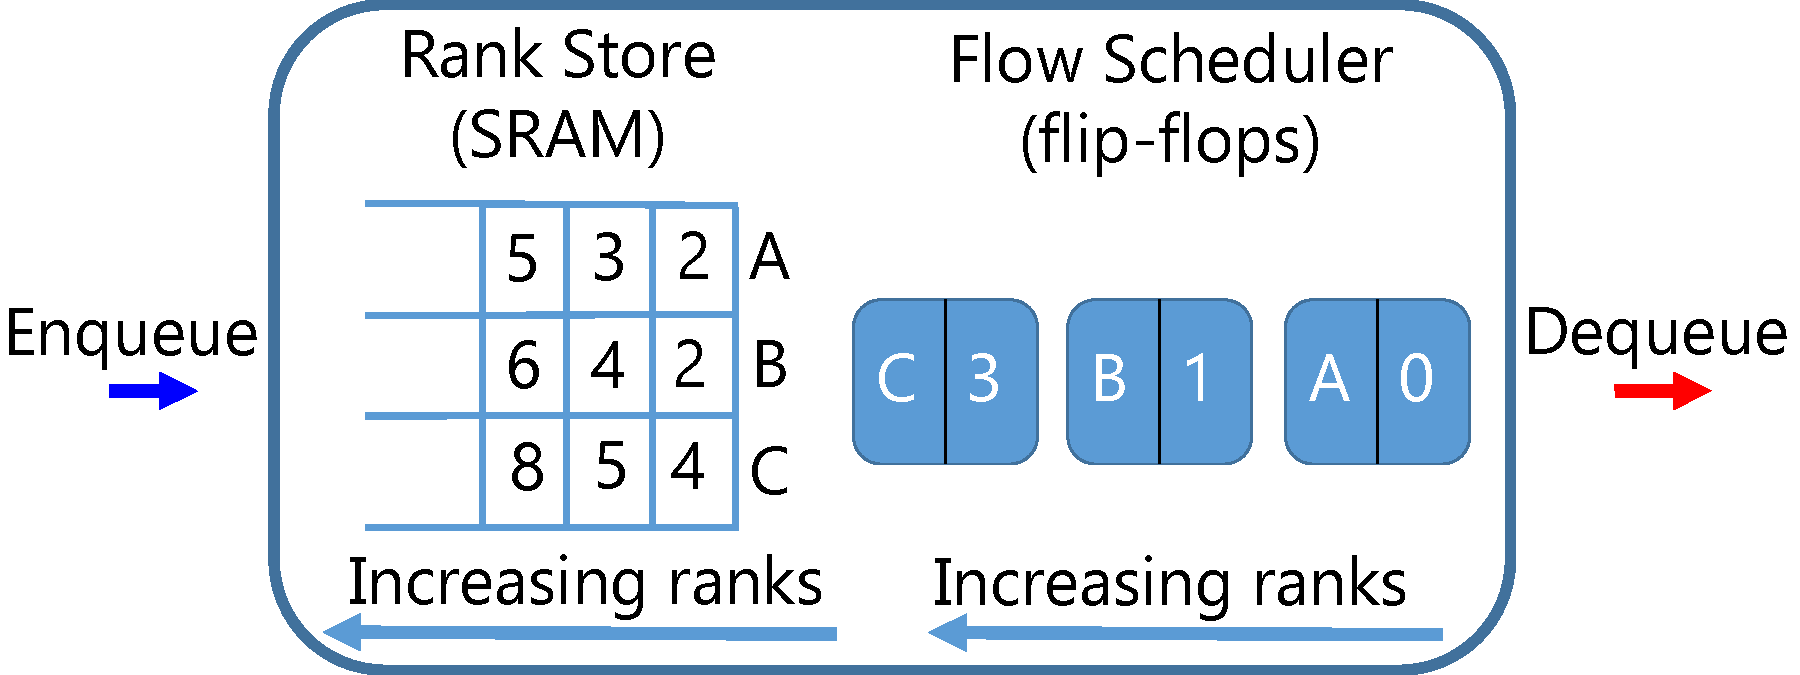
\includegraphics[width=0.6\columnwidth]{pifo_pifo_impl.pdf}
  \caption{Block diagram of PIFO block with a flow scheduler and a
   rank store. Logical PIFOs and metadata are not shown for simplicity.}
  \label{fig:pifo_impl}
\end{figure}

This decomposition reduces the number of elements requiring sorting from the
number of packets (64K) to the number of flows (1024). Maintaining a flat
sorted array of 1024 elements turns out to be much more feasible in today's
transistor technology.

During an enqueue, an element (both rank and metadata) is appended to the end
of the appropriate FIFO in the rank store. For a flow's first element, we
bypass the rank store and directly push it into the flow scheduler. To permit
enqueues into this PIFO block, we also supply a flow ID argument to the enqueue
operation. During dequeues, we dequeue the element with the earliest rank among
the head elements of all flows in the flow scheduler.  We then insert the next
element after the head for the flow that was just dequeued.

The FIFO bank needed for the rank store is a well understood hardware design.
Such FIFO banks are used to buffer packet payloads in router queues and
substantial engineering effort has gone into optimizing them.  As a result, we
focus our discussion here on the flow scheduler alone.

\Para{The flow scheduler.}
The flow scheduler sorts an array of flows using the ranks of the head elements
of all flows. It supports one enqueue {\em and} one dequeue to its enclosing
PIFO block every clock cycle, which translates into the following operations on
the flow scheduler every clock cycle.
\begin{CompactEnumerate}
  \item Enqueue operation: Inserting a flow into the flow scheduler 
  when the flow goes from empty to non-empty.
\item Dequeue operation: Removing a flow from the flow scheduler that empties
once it is scheduled, (or) removing and reinserting a flow into the flow
scheduler with the rank of the next element if the flow is still backlogged.
\end{CompactEnumerate}

The operations above require the flow scheduler to internally support two kinds
of operations every clock cycle.
\begin{CompactEnumerate}
\item {\em Push} up to two elements into the flow scheduler: one each for an
  enqueue's insert and a dequeue's reinsert.
\item {\em Pop} one element: for the removal of a flow because of a dequeue.
\end{CompactEnumerate}
These internal operations access all of the flow scheduler's elements in
parallel. To facilitate this, we implement the flow scheduler in flip flops,
unlike the rank store, which is in SRAM.

The flow scheduler is organized in hardware as a sorted array, where a push is
implemented by executing the three steps below
(Figure~\ref{fig:flow_scheduler}).
\begin{CompactEnumerate}
\item Compare the incoming rank against all ranks in the array in parallel using a comparator.
  This produces a bit mask of comparison results indicating if the incoming rank
  is greater/less than an array element's rank.
\item Find the first 0-to-1 transition in this bit mask, using a priority encoder. The location of this transition determines the index to push into.
\item Push the element into this index, by shifting the array.
\end{CompactEnumerate}
A pop is implemented by shifting the head element out of the sorted array.

\begin{figure}[!t]
  \centering
  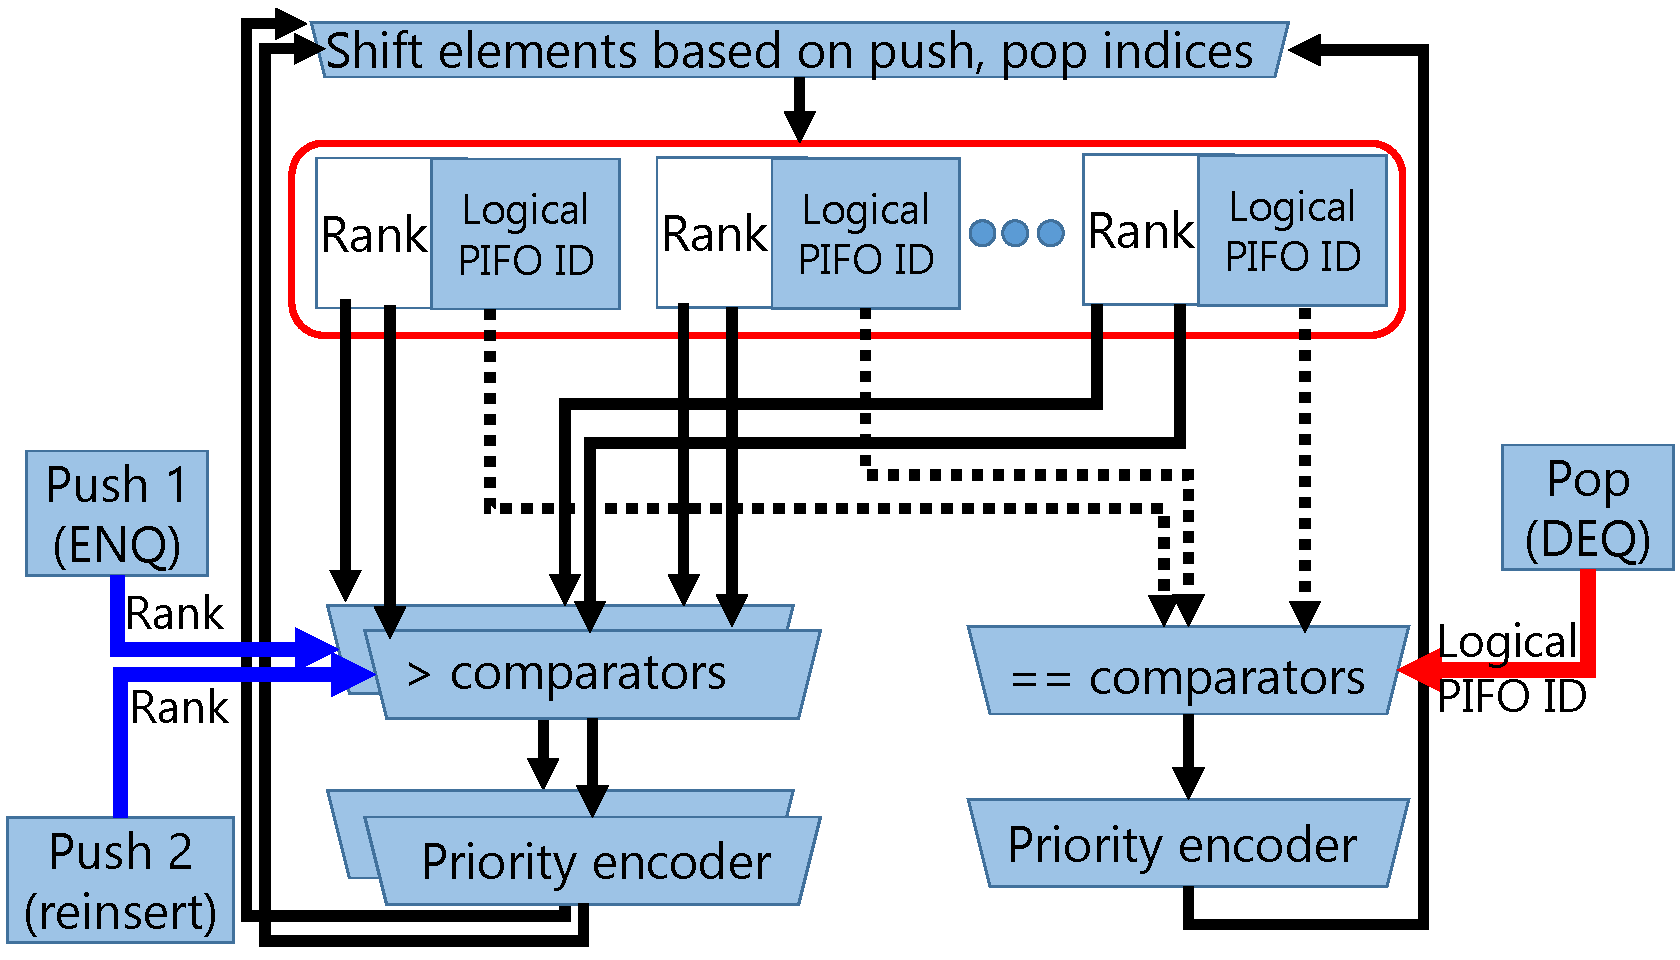
\includegraphics[width=0.6\columnwidth]{pifo_flow_scheduler_hardware.pdf}
  \caption{Hardware implementation of flow scheduler. Each element in the flow
  scheduler is connected to two > comparators (2 pushes) and one == comparator (1
  pop).}
  \label{fig:flow_scheduler}
\end{figure}

\begin{figure}[!t]
  \centering
  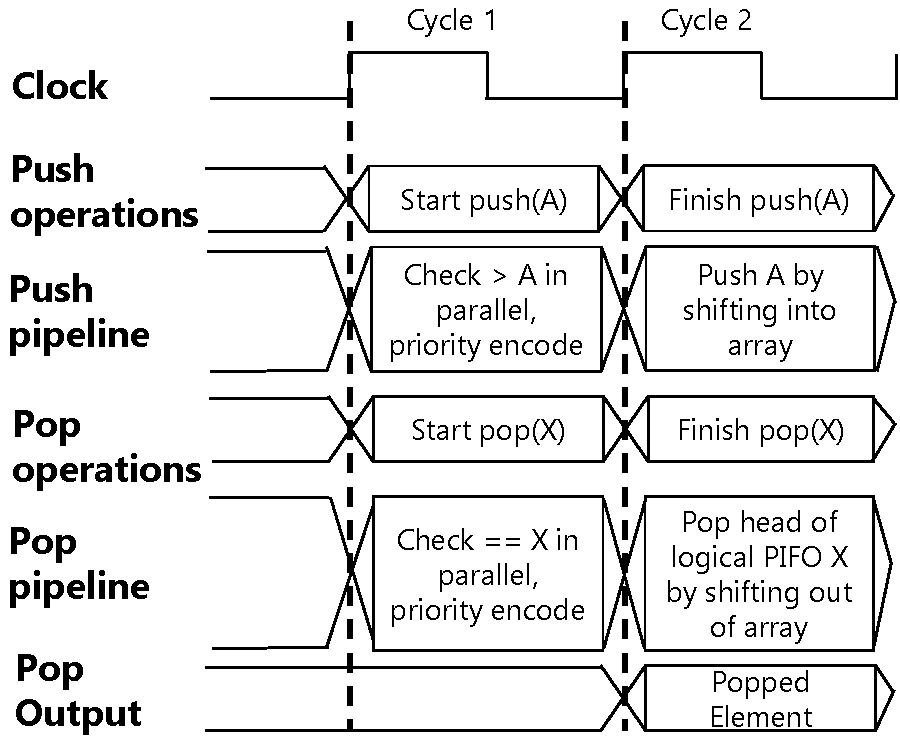
\includegraphics[width=0.6\columnwidth]{pifo_2stage_pipeline.pdf}
  \caption{2-stage pipeline for flow scheduler}
  \label{fig:2stage}
\end{figure}



So far, we have focused on a flow scheduler implementation handling a single
logical PIFO. We can extend this to handle multiple logical PIFOs backed by the
same underlying physical hardware. To do so, we keep elements sorted by rank,
regardless of the logical PIFO they belong to; hence, the push logic does not
change.  To pop from a specific logical PIFO, we compare the dequeue's logical
PIFO ID against all elements to find elements with that logical PIFO ID alone.
Among these elements, we find the first using a priority encoder, and remove
this element by shifting the array.  The rank store implementation does not
change when introducing logical PIFOs; however, we do require that a flow
belong to exactly one logical PIFO.

Recall that to support one enqueue and one dequeue every clock cycle, the flow
scheduler needs to support 2 pushes and 1 pop every clock cycle. To concurrently
issue 2 pushes and 1 pop every clock cycle, we provision 3 parallel digital circuits
(Figure~\ref{fig:flow_scheduler}). Both the push and pop require 2 clock cycles to
complete and need to be pipelined to maintain the required throughput
(Figure~\ref{fig:2stage}). For pushes, the first stage of the pipeline executes
the parallel comparison and priority encoder steps to determine an index; the
second stage pushes the element into the array using the index.  Similarly, for
pops, the first stage executes the equality check (for logical PIFO IDs) and
priority encoder steps to compute an index; the second stage pops the head
element out of the array using the index.

Our implementation meets timing at 1 GHz and supports up to one enqueue/dequeue
operation on a logical PIFO within a PIFO block every clock cycle. Because a reinsert
operation requires a pop, followed by an access to the rank store for the next
element, followed by a push, our implementation supports a dequeue from the
same logical PIFO only once every 4 clock cycles. This is because if a dequeue is
initiated in clock cycle 1, the pop for the dequeue completes in 2, the rank
store is accessed in 3, and the push is initiated in 4. This makes clock cycle 5 the
earliest time to reissue a dequeue.  This restriction is inconsequential in
practice.  A dequeue every 4 clock cycles from a logical PIFO is sufficient to
service the highest link speed today, 100 Gbit/s, which requires a dequeue at
most once every 5 clock cycles for a minimum packet size of 64 bytes. Dequeues
to distinct logical PIFO IDs are still permitted every clock cycle.

\subsection{Interconnecting PIFO blocks}
\label{ss:interconnect}

An interconnect between PIFO blocks allows PIFO blocks to enqueue into and
dequeue from other blocks. Because the number of PIFO blocks is small, we
provide a full mesh between them. For a 5-block PIFO mesh as in our baseline
design, this requires 5*4 = 20 sets of wires between PIFO blocks. Each set
carries all the inputs required for specifying an enqueue and dequeue operation
on a PIFO block.

We now calculate the size of the inputs required to specify enqueue and dequeue
operations.  For our baseline design (\S\ref{ss:performance}), for an enqueue,
we require a logical PIFO ID (8 bits), the element's rank (16 bits), the
element meta data (32 bits), and the flow ID (10 bits). For a dequeue, we need
a logical PIFO ID (8 bits) and wires to store the dequeued element's metadata
field (32 bits).  Combining both enqueue and dequeue, this adds up to 106 bits
per set of wires, or 2120 bits for the mesh. This is a small number of wires
for an entire chip.  For example, RMT's match-action pipeline uses 4000 1-bit
wires between a {\em a pair of pipeline stages} to move its 4K packet header
vector between stages~\cite{rmt}. 

\subsection{Area overhead}
\label{ss:feasibility}

Because we target a single-pipeline router, the scheduling logic is shared
across all ports and a single PIFO mesh services an entire router.  Therefore,
to estimate the area overhead of a programmable scheduler, we estimate the area
overhead of a single PIFO mesh. Our overhead does not have to be multiplied by
the number of ports and is the same for two single-pipeline routers with equal
aggregate packet rates, \eg a 6-port 100G router and a 60-port 10G router.

To determine the area of a PIFO mesh, we compute the area of a single PIFO
block and multiply it by the number of blocks because the area of the
interconnect itself is negligible (\S\ref{ss:interconnect}).  For a single
block's area, we separately estimate areas for the rank store, atom pipelines,
and flow scheduler. We ignore the area of the small next-hop lookup tables.  We
estimate the rank store's area by using SRAM estimates~\cite{sram_estimate} and
the atom pipeline's area using the individual atom area numbers from
Table~\ref{tab:templates}. We estimate the flow scheduler's area by
implementing it in Verilog~\cite{system_verilog} and synthesizing it to a
gate-level netlist in a 16-nm standard cell library using the Cadence Encounter
RTL Compiler~\cite{cadence_rc}. The RTL Compiler also verifies that the flow
scheduler meets timing at 1 GHz.

Overall, our baseline design consumes about 7.35 \si{\milli\metre\squared} of
chip area (Table~\ref{tab:area_overheads}). This is about 3.7\% of the chip
area of a router chip, using the minimum chip area estimate of 200
\si{\milli\metre\squared} provided by Gibb et al.~\cite{glen_parsing}. In
return for this 3.7\%, we get a significantly more flexible packet scheduler
than current routers, which provide {\em fixed} two or three-level hierarchical
scheduling. Our 3.7\% area overhead is similar to the overhead for other
programmable router functions, \eg 2\% for programmable
parsing~\cite{glen_parsing} and 15\% for programmable header
processing~\cite{rmt}.
 
\begin{table}[!h]
  \centering
  \begin{small}
  \begin{tabular}{|p{0.36\textwidth}|p{0.5\textwidth}|}
  \hline
  Component & Area in \si{\milli\metre\squared}\\
  \hline
  Router chip & 200--400~\cite{glen_parsing} \\
  \hline
  Flow Scheduler & 0.224 (from synthesis) \\
  \hline
  SRAM (1 Mbit) & 0.145~\cite{sram_estimate} \\
  \hline
  Rank store & 64 K * (16 + 32) bits * 0.145 \si{\milli\metre\squared} / Mbit = 0.445 \\
  \hline
  Next pointers for linked lists in dynamically allocated rank store & 64 K * 16 bit pointers * 0.145 = 0.148 \\
  \hline
  Free list memory for dynamically allocated rank store & 64 K * 16 bit pointers * 0.145 = 0.148 \\
  \hline
  Head, tail, and count memory for each flow in the rank store & 0.1476 (from synthesis) \\
  \hline
  One PIFO block & 0.224 + 0.445 + 0.148 + 0.148 + 0.1476 = 1.11 \si{\milli\metre\squared} \\
  \hline
  5-block PIFO mesh & 5.55 \\
  \hline
  300 atoms spread out over the 5-block PIFO mesh for rank computations & 6000 \si{\micro\metre\squared}* 300 = 1.8 \si{\milli\metre\squared} (\S\ref{ss:transactions},~Table~\ref{tab:templates})\\
  \hline
  Overhead for 5-block PIFO mesh & (5.55 + 1.8) / 200.0 = 3.7 \% \\
  \hline
  \end{tabular}
\end{small}
\caption{A 5-block PIFO mesh needs 3.7\% additional chip area relative to
a baseline router.}
\label{tab:area_overheads}
\end{table}

\begin{table}
\centering
\begin{small}
\begin{tabular}{|p{0.1\textwidth}|p{0.1\textwidth}|p{0.2\textwidth}|}
\hline
\# of flows & Area (mm\textsuperscript{2}) & Meets timing at 1 GHz? \\
\hline
256 & 0.053 & Yes \\
\hline
512 & 0.107 & Yes \\
\hline
1024 & 0.224 & Yes \\
\hline
2048 & 0.454 & Yes \\
\hline
4096 & 0.914 & No \\
\hline
\end{tabular}
\end{small}
\caption{The flow scheduler's area increases with the number of
flows. The flow scheduler meets timing until 2048 flows.}
\label{tab:num_flows}
\end{table}

\Para{Varying the flow scheduler's parameters from the baseline.}
The flow scheduler has four parameters: rank width, metadata width, number of
logical PIFOs, and number of flows. Among these, increasing the number of flows
has the most impact on whether the flow scheduler meets timing at 1 GHz.  This
is because the flow scheduler uses a priority encoder, whose size is
the number of flows and whose critical path delay increases with the number of
flows. With other parameters set to their baseline values, we vary the number
of flows to determine the eventual limits of a flow scheduler with today's
transistor technology (Table~\ref{tab:num_flows}), and find that we can scale
to 2048 flows while still meeting timing at 1 GHz.

The remaining parameters affect the area of a flow scheduler, but have
little effect on meeting timing at 1 GHz. For instance, starting from
the baseline design of the flow scheduler that takes up 0.224
\si{\milli\metre\squared}, increasing the rank width to 32 bits increases it
 to 0.317 \si{\milli\metre\squared}, increasing the number of logical
PIFOs to 1024 increases it to 0.233 \si{\milli\metre\squared}, and
increasing the metadata width to 64 bits increases it to 0.317
\si{\milli\metre\squared}. In all cases, the flow scheduler continues to meet timing.

% Technically, the critical path delay is proportional to:
% 1. log of metadata width
% 2. log of rank width
% 3. log of logical PIFO width, \ie log(log(number of logical PIFOs))
% 4. log of number of PIFOs.
% 4 grows fastest in practice, though theoretically, 1, 2, and 4 have the same order of growth.

\subsection{Additional implementation concerns}
\label{ss:add_impl}

\Para{Coordination between enqueue and dequeue.}
When computing packet ranks on enqueue, some scheduling algorithms access state
modified on packet dequeues. An example is STFQ (\S\ref{ss:wfq}) that accesses
the \texttt{virtual\_time} variable when computing a packet's virtual start
time. This enqueue-dequeue coordination can be implemented in two ways.  One is
shared state that can be accessed on both enqueue and dequeue, similar to queue
occupancy counters. Another is to periodically synchronize the enqueue and
dequeue views of the same state, potentially by creating and recirculating a
packet carrying this information from the dequeue to the enqueue pipeline.  For
STFQ, the degree of short-term fairness is directly correlated with how
up-to-date the \texttt{virtual\_time} information on the enqueue side is.

\Para{Buffer management.}
Our design focuses on programmable scheduling and does not manage the
allocation of a router's data buffer across flows.  Buffer management can use
static buffer limits for each flow. The limits can also be dynamic, \eg
RED~\cite{red} and dynamic buffer sizing~\cite{broadcom_dynamic}.

In a single-pipeline shared-memory router, buffer management is orthogonal to
scheduling, and is implemented using counters that track flow occupancy in a
shared buffer. Before a packet is enqueued into the scheduler, if any counter
exceeds a static or dynamic threshold, the packet is dropped. A similar design
for buffer management could be used with a PIFO-based scheduler as well.

\Para{Priority Flow Control.}
Priority Flow Control (PFC)~\cite{pfc} is a standard that allows a router to
send a {\em pause} message to an upstream router requesting it to cease
transmission of packets belonging to particular flows. PFC can be integrated
into our hardware design by excluding certain flows in the flow scheduler
during the dequeue operation if they have been paused because of a PFC pause
message. These flows can be included again when a PFC {\em resume} message is
received.  This exclusion-inclusion process can be accomplished by using a
bitmask to indicate which flows are currently excluded or included and ANDing
with this bitmask when dequeueing from the flow scheduler.
